\documentclass[11pt,notitlepage,a4paper]{article}

\usepackage[left=2cm,right=2cm,top=2cm,bottom=2cm]{geometry}
\usepackage{graphicx}
%%BeginIpePreamble
\usepackage{amssymb,mathtools, amsmath, amsfonts, amsthm}
%%EndIpePreamble
%\usepackage{color}
\usepackage{float}
\usepackage{hyperref}
\usepackage{enumerate}
\usepackage{enumitem}
\usepackage{chngcntr}
\usepackage{cleveref}
\usepackage{pdfpages}
\usepackage{caption,subcaption,float}

\counterwithout{equation}{section}



\newlength{\margen}
\setlength{\margen}{\paperwidth}
\addtolength{\margen}{-\textwidth}
\addtolength{\skip\footins}{0.7 cm}
\setlength{\margen}{0.5\margen}
\addtolength{\margen}{-1in}
\setlength{\oddsidemargin}{\margen}
\setlength{\evensidemargin}{\margen}
\setlength{\abovedisplayskip}{3pt}
\setlength{\belowdisplayskip}{3pt}
%%%% Small setup %%%%
\hypersetup{
	colorlinks=false,
	pdfborder={1 1 0.0005},
}
\setlength{\parskip}{0.2cm}
%%%%%%%%%%%%%%%
%\usepackage{tikz-cd}
%\usetikzlibrary{cd}
\usepackage[english]{babel}
%\usepackage{todonotes}
%\usepackage{cleveref}
%\usepackage{caption}
%\usepackage{subcaption}
%\usepackage{bbding}
%\usepackage{tcolorbox}
%\usepackage{natbib}
%
%\DeclareMathOperator{\incl}{incl}

\newtheorem{proposition}{Proposition}[section]
\newtheorem{fact}{Fact}[section]
\newtheorem{theorem}{Theorem}[section]
\newtheorem{lemma}{Lemma}[section]
\newtheorem{corollary}{Corollary}[section]
\theoremstyle{definition}
\newtheorem{definition}{Definition}[section]
\newtheorem{propdef}{Proposition / Definition}[section]
\newtheorem{remark}{Remark}[section]
\newtheorem*{lemma*}{Lemma}
\newtheorem*{claim*}{Claim}

%
%\newtheorem{inneraxiom}{Axiom}
%\newenvironment{axiom}[1]
%{\renewcommand\theinneraxiom{#1}\inneraxiom}
%{\endinneraxiom}
%\newcommand{\cc}{\mathfrak{c}}


%\newcommand{\Hc}{\mathcal{H}}
%\newcommand{\Lan}{\mathcal{L}}
%
%\newcommand{\clist}{\mathfrak{c}_{1}, \cdots, \mathfrak{c}_m}
%\newcommand{\morph}[1]{\stackrel{#1}{\simeq}}
%\newcommand{\vlst}[2]{#1_1,\dots, #1_{#2}}
%\newcommand{\gnp}{G(n,\beta_1/n^{a_1-1}, \dots,\beta_l/n^{a_l-1})}
\newcommand{\Z}{\mathbb{Z}}
\newcommand{\CC}{\mathbb{C}}
\newcommand{\Q}{\mathbb{Q}}
\newcommand{\R}{\mathbb{R}}
\newcommand{\N}{\mathbb{N}}
\DeclarePairedDelimiter\floor{\lfloor}{\rfloor}
\newcommand{\Ln}{\lim\limits_{n\to \infty}}

\title{Proof Sketches Regarding the Closure of 
	Limiting Probabilities in Sparse Random Hyper-graphs}
\date{\today}
\author{Alberto Larrauri}


\begin{document}
	\maketitle
	
\section*{Preliminaries}

Let $G^d(n,p)$ denote the binomial random $d$-uniform hyper-graph on $n$ 
vertices where each edge has probability $p$. We are interested in 
the case where $p=\frac{c}{n^{d-1}}$ for some non-negative real constant $c$.
\par
For the remainder of this writing we will work with $d$-uniform hyper-graphs
with $d\geq 3$ some fixed number. We will abbreviate ``$d$-uniform hyper-graph"
as ``graph".
\par

We will call the \textbf{fragment} $F_n$ to the union of the unicyclic 
components in $G^d(n,c/n^{d-1})$. In this setting, a unicycle is a connected
graph $H$ such that $(d-1)e(H)-v(H)=0$. 
\par


We can show that for $0\leq c \leq (d-2)!$
\[ \Ln \mathrm{Pr}\big( F_n \text{ is empty }\big)= e^{\frac{c}{2(d-2)!}}\sqrt{1 - c/(d-2)!}.\]

Instead of working with $c$ it is more convenient to use $r:= c/(d-2)!$
as our parameter. We will denote the RHS of last equation as $A(r)$. 
The limit probability $A(r)$ that a graph is acyclic reaches $1/2$ when
$r=0.898172...$.\par

Given any graph $H$ which is a disjoint union of unicycles, 
for $0\leq r < 1$ it is satisfied
\begin{equation} \label{probformula}
\Ln \mathrm{Pr}\big( F_n\simeq H \big)= A(r)(re^{-r})^{e(H)}
\frac{(d-2)!^{e(H)}}{|Aut(H)|},
\end{equation}
where $Aut(H)$ denotes the group of automorphisms of $H$.  \par 

\section*{For $0.898172...\leq r < 1$ there are no gaps}

Fix $0.898172...\leq r < 1$.
Let $H_0,H_1,\dots$ be an enumeration of all graphs with 
unicyclic components such that $p_0 \leq p_1 \leq \dots$,
where $p_i$ is the limit probability that the fragment 
$F_n$ is isomorphic to $H_i$, given by \cref{probformula}.
We want to show that
\begin{equation} \label{eqn:kakeya}
	p_i \leq \sum_{j>i} p_j \qquad \forall i.
\end{equation} 
\par
Let $q_i=p_i/A(r)$ and let $s=re^{-r}$. Then
 \[ q_i= s^{e(H_i)}
 \frac{(d-2)!^{e(H_i)}}{|Aut(H_i)|},
 \]
and \cref{eqn:kakeya} holds iff
\begin{equation} \label{eqn:kakeya2}
q_i \leq \sum_{j>i} q_j \qquad \forall i. 
\end{equation}

\par

We will call a vertex $v\in V(H)$ \textbf{free} if it belongs 
to exactly one edge in $H$. Free vertices inside an edge are
indistinguishable, so 
	\[	\prod_{h\in E(H)} |Free(h)|! \leq |Aut(H)|, \]
where $Free(h)$ denotes the number of free vertices in the edge $h$.\par
We call an edge $e\in E(H)$ a \textbf{leaf} if it only contains one
non-free vertex.  
\par
The following lemma is not strictly necessary. It will be only used once
and its use could have been avoided in exchange of doing a more exhaustive
enumeration of graphs so maybe that is the preferable option. 

\begin{lemma*} For any graph $H$ whose connected components are 
	unicycles,
	\[ \frac{(d-2)!^{e(H)}}{|Aut(H)|} \leq \frac{(d-2)^2}{(d-1)^2}.\]
\end{lemma*}
\begin{proof}
%	We have two cases. If $H$ is the cycle of length 
%	$l\geq 2$ then $|Aut(H)|=(d-2)!^l 2l$, and
%	\[ \frac{(d-2)!^{e(H)}}{|Aut(H)|}=\frac{1}{2l} 
%	\leq \frac{(d-2)^2}{(d-1)^2},\]
%	as $1/2l\leq 1/4 \leq (d-2)^2/(d-1)^2$ for all 
%	$l\geq 2, d\geq 3$. 
%	\par
%	Otherwise $H$ is a cycle with some trees attached to it. We
%	will prove the statement for these unicycles using an inductive
%	argument. \par
	It suffices to prove the statement for unicycles, because
	 \[ \frac{(d-2)!^{e(H)}}{|Aut(H)|}\leq \prod_{i} \frac{(d-2)!^{e(H_i)}}{|Aut(H_i)|}, \]
	where the $H_i$'s are the connected components of $H$.\par
	Let $\lambda=\lambda(H)$ be the number of 
	leaves in $H$. We show by induction that
	\begin{equation}\label{ineqleaves}
	\prod_{h\in E(H)} \frac{(d-2)!}{|Free(h)|!} \leq 
	\left(\frac{d-2}{d-1}\right)^\lambda.
	\end{equation}
	\par
	If $\lambda=0$ then $H$ is a cycle and each one of
	its edges contains exactly $d-2$ free vertices, so
	\[	\prod_{h\in E(H)} \frac{(d-2)!}{|Free(h)|!}=1=
	\left(\frac{d-2}{d-1}\right)^0.\]
	And $H$ satisfies \cref{ineqleaves}.
	\par
	Now let $H$ be an unicycle satisfying 
	\cref{ineqleaves}. Add a new edge $h^\prime$ to $H$ 
	to obtain another unicycle $H^\prime$. Then 
	$h^\prime$ intersects $H$ in only one vertex $v$. 
	In consequence $h^\prime$ is a leave of $H^\prime$.
	\par
	Consider the case $\lambda(H^\prime)=\lambda(H)$,
	where no new leaves are created with the addition of
	$h^\prime$. This means that $v$ is a free vertex in one
	leaf $f$ of $H$ (that is, $h^\prime$ ``grows" out of $f$), 
	and
	\[	\prod_{h\in E(H^\prime)} \frac{(d-2)!}{|Free(h)|!}=
	\prod_{h\in E(H)} \frac{(d-2)!}{|Free(h)|!}.\]
	\par
	Otherwise $\lambda(H^\prime)=\lambda(H)+1$. In this case
	$h^\prime$ intersects an edge of $H$ that is not a leaf.
	Here, the case that maximizes $\prod_{h\in E(H^\prime)} 
	\frac{(d-2)!}{|Free(h)|!}$ is the one where $h^\prime$ grows out  
	of a free vertex of an edge in $H$ with exactly
	$d-2$ free vertices. In this case
	\[	\prod_{h\in E(H^\prime)} \frac{(d-2)!}{|Free(h)|!}=
	\frac{d-2}{d-1} \prod_{h\in E(H)} 
	\frac{(d-2)!}{|Free(h)|!},\]
	and $H^\prime$ satisfies \cref{ineqleaves} as well.\par
	Finally, as all unicycles can be obtained adding edges
	to a cycle successively, \cref{ineqleaves} holds for all
	unicycles. \par
	To prove the original statement consider the cases 
	$\lambda=0, \lambda=1$ and $\lambda\geq 2$. If 
	$\lambda=0$ then $H$ is a cycle of length $l\geq 2$ 
	and $|Aut(H)|=(d-2)!^l 2l$, yielding
	\[ \frac{(d-2)!^{e(H)}}{|Aut(H)|}=\frac{1}{2l} 
	\leq \frac{(d-2)^2}{(d-1)^2},\]
	as $1/2l\leq 1/4 \leq (d-2)^2/(d-1)^2$ for all 
	$l\geq 2, d\geq 3$.
	\par
	If $\lambda=1$ then $H$ is a cycle with a path attached
	to it. In this case, there is a reflection of the cycle 
	of $H$ in $Aut(H)$, and in consequence 
	$2\prod_{h\in E(H)} |Free(h)|! \leq |Aut(H)|$. Using this
	and \cref{ineqleaves} we get
	\[ \frac{(d-2)!^{e(H)}}{|Aut(H)|}\leq \frac{1}{2}
	\prod_{h\in E(H)} \frac{(d-2)!}{|Free(h)|!}\leq
	\frac{1}{2} \left( \frac{d-2}{d-1}\right)\leq
	\left( \frac{d-2}{d-1}\right)^2,	
	\]
	as we wanted.\par
	Finally, for the case $\lambda \geq 2$ just \cref{ineqleaves}
	suffices, as
	\[
	\prod_{h\in E(H)} \frac{(d-2)!}{|Free(h)|!}\leq
	\left( \frac{d-2}{d-1}\right)^\lambda \leq
	\left( \frac{d-2}{d-1}\right)^2.	
	\]
	 
	
	
%	We can improve last bound using the following consideration.
%	Each automorphism of $H$ induces a permutation on the edge set
%	$E(H)$. Let $Aut_E(H)$ denote the group of such permutations of 
%	$E(H)$. Now notice that if an automorphism $\phi\in Aut(H)$
%	induces an edge permutation $\phi_E \in Aut_E(H)$, then composing
%	$\phi$ with all the allowed permutations of free vertices of $H$
%	yields $\prod_{h\in E(H)} |Free(h)|!$ different automorphisms
%	of $H$, and all of those automorphisms induce $\phi_E$. 
%	In consequence	
%	\[	|Aut_E(J)| \prod_{h\in E(H)} |Free(h)|! \leq |Aut(H)|. \]
	
	
	
%	\par
%	If $H$ is a cycle with an extra edge attached to it
%	then $\prod_{h\in E(H)} \frac{(d-2)!}{|Free(h)|!}$ equals either
%	$\frac{1}{d-1}$ or $\frac{d-2}{d-1}$, so the statement holds. 
%	\par
%	Now, assume that $H$ is an unicycle such that 
%	$\prod_{h\in E(H)} \frac{(d-2)!}{|Free(h)|!}
%	\leq \frac{d-2}{d-1}$.
%	Add a new edge $h^\prime$ 
%	to $H$ to obtain a new unicycle $H^\prime$. This way,
%    \[\prod_{h\in E(H^\prime)\setminus \{h^\prime \}} 
%	\frac{(d-2)!}{|Free(h)|!} \leq (d-1) \prod_{h\in E(H)} 
%	\frac{(d-2)!}{Free(h)|!}\leq d-2. \]
%	Here the first inequality is derived from the fact that 
%	with the addition of $h^\prime$, the edges in $H$ lose at 
%	most one free vertex in total. Now, using the fact that
%	$h^\prime$ contains exactly $d-1$ free vertices we get
%	\[\prod_{h\in E(H^\prime)} 
%	\frac{(d-2)!}{|Free(h)|!} \leq (d-2)
%	\frac{(d-2)!}{|Free(h^\prime)|!} = \frac{d-2}{d-1}, \]
%	as we wanted to prove. 
\end{proof} 
 
The bound in last lemma can be reached. Consider the 
family of graphs $(T_{\alpha,\beta})$, for $\alpha,\beta>0$,
where $T_{\alpha,\beta}$ denotes the graph consisting of
a triangle with two paths of length $\alpha$ and $\beta$ 
respectively attached to two of its free vertices, 
each one from a different edge. One can check
\[
\frac{(d-2)!^{e(T_{\alpha,\beta})}}{|Aut(T_{\alpha,\beta})|}=
\frac{(d-2)!^{\alpha+\beta+3}}{|Aut(T_{\alpha,\beta})|}=\begin{cases}
\left(\frac{d-2}{d-1}\right)^2 \text{ for } \alpha\neq\beta \text{,   or}\\
\\
\frac{1}{2}\left(\frac{d-2}{d-1}\right)^2\text{ otherwise.} 
\end{cases}
\]
Then, for $k\geq 4$, if we sum $\frac{(d-2)!^{k}}
{|Aut(H)|}$ for all different graphs with $k$ edges
of the form $T_{\alpha,\beta}$ we obtain 
\begin{equation} \label{eqn:triangles}
 \sum_{\alpha=1}^{\floor*{\frac{k-3}{2}}}
\frac{(d-2)!^{k}}{|Aut(T_{\alpha,k-3-\alpha})|}= 
\frac{k-4}{2} \left( \frac{d-2}{d-1} \right)^2
\end{equation}
using considerations similar to the ones
in the sketches of Tobias. \par

We introduce now another two families of graphs. \par

The graph $B_{\alpha,\beta}$, for $\alpha,\beta>0$, is
the one consisting of a two-cycle with two paths 
of length $\alpha$ and $\beta$ 
respectively attached to two of its free vertices, 
each one from a different edge. In this case

\[
\frac{(d-2)!^{e(B_{\alpha,\beta})}}{|Aut(B_{\alpha,\beta})|}=
\frac{(d-2)!^{\alpha+\beta+2}}{|Aut(B_{\alpha,\beta})|}=
\begin{cases}
\frac{1}{2}\left(\frac{d-2}{d-1}\right)^2 
\text{ for } \alpha\neq\beta \text{,   or}\\
\\
\frac{1}{4}\left(\frac{d-2}{d-1}\right)^2\text{ otherwise.} 
\end{cases}
\]

Summing $\frac{(d-2)!^{k}}{|Aut(H)|}$ for all different
graphs of the form $B_{\alpha,\beta}$ with $k\geq 3$ edges
yields
\begin{equation}  \label{eqn:twocycles}
\sum_{\alpha=1}^{\floor*{\frac{k-2}{2}}}
\frac{(d-2)!^{k}}{|Aut(T_{\alpha,k-2-\alpha})|}= 
\frac{k-3}{4}\left( \frac{d-2}{d-1} \right)^2
\end{equation}
\par
We define the graph $O_{\alpha,\beta}$,
with $\alpha>1, \beta>0$, as the one
formed by attaching a path of length
$\beta$ to a free vertex of a cycle of
length $\alpha$. One can check that 
$e(O_{\alpha,\beta})=\alpha+\beta$ and
that $\frac{(d-2)!^{\alpha+\beta}}
{|Aut(O_{\alpha,\beta})|}=
\frac{1}{2}\left(\frac{d-2}{d-1}\right)$.
In consequence, summing $\frac{(d-2)!^{k}}{|Aut(H)|}$
for all different graphs of the form $O_{\alpha,\beta}$ 
with $k\geq 2$ edges we obtain

\begin{equation}  \label{eqn:cycles}
\sum_{\alpha=2}^{k-1}
\frac{(d-2)!^{k}}{|Aut(O_{\alpha,k-\alpha})|}= 
\frac{k-2}{2}\left( \frac{d-2}{d-1} \right).
\end{equation}

\par






%$(O_{\alpha,\beta})$ with $\alpha\geq 2$, $\beta\geq 1$,
%where $O_{\alpha,\beta}$ is the graph obtained by attaching a path
%of length $\beta$ to a cycle of length $\alpha$ in a way such that
%no vertex belongs to three edges. Then
%\[
%\frac{(d-2)!^{e(O_{\alpha,\beta})}}{|Aut(O_{\alpha,\beta})|}=
%\frac{(d-2)!^{\alpha+\beta}}{|Aut(O_{\alpha,\beta})|}=\begin{cases}
%\frac{1}{2} \frac{(d-2)}{(d-1)} \text{ for } \alpha=2,3 \text{,   or}\\
%\\
%\frac{d-2}{d-1} \text{ otherwise.} 
%\end{cases}
%\]

For any $i\in \N$, let $k=k(i)$ be the natural number such that
\[
s^{k-1} \left(\frac{d-2}{d-1}\right)^2 \geq q_i > s^k 
\left(\frac{d-2}{d-1}\right)^2
\]
Notice that because of our previous lemma
$k(i)-1\geq e(H_i)$. \par
Let $\mathcal{U}_k$ be the set of unlabeled graphs with $k$ 
edges whose components are unicycles. We will show that
\cref{eqn:kakeya2} is satisfied for the different possible
values of $k(q_i)$. \par

If $k\geq 4$ then 
\[ s^k \sum_{H\in U_k}\frac{(d-2)!^k}{|Aut(H)|} 
\geq s^k\left[\frac{k-4}{2} \left( \frac{d-2}{d-1} \right)^2 +
\frac{k-2}{2} \left( \frac{d-2}{d-1} \right)\right] \geq 
s^k (k-3) \left( \frac{d-2}{d-1} \right)^2.
\]

This is obtained taking into account the graphs of the form
$T_{\alpha,\beta}$ and $O_{\alpha,\beta}$ in $\mathcal{U}_k$ and
using \cref{eqn:triangles} and \cref{eqn:triangles}.\par

Using last inequality and that
$1/3 < s$, if $k=k(i)\geq 6$ then
\[\sum_{j>i}^{q_i}>
s^k\sum_{H\in U_k}\frac{(d-2)!^k}{|Aut(H)|}
> s^k(k-3) \left( \frac{d-2}{d-1} \right)^2
> s^{k-1} \left( \frac{d-2}{d-1} \right)^2 > q_i.
\]

If $k=k(i)=5$ then
\[\sum_{j>i}^{q_i}>
s^5\sum_{H\in U_5}\frac{(d-2)!^5}{|Aut(H)|}
+ s^6\sum_{H\in U_6}\frac{(d-2)!^6}{|Aut(H)|}
> (s^52 + s^63) \left( \frac{d-2}{d-1} \right)^2 
> s^4 \left( \frac{d-2}{d-1} \right)^2 \geq q_i.
\]

\par

The only cases left are $k(i)=4$ and $k(i)=3$. 
We will study them together. \par
Assume $k(i)\leq 4$. Then $e(H_i)\leq 3$ 
(this is the only place where we 
really use the lemma).
If $e(H_i)=3$ then an enumeration
of all unicycles with three edges gives $q_i 
\leq s^{3}\frac{1}{2} \left( \frac{d-2}{d-1} \right)$. \par
\begin{figure}[H]
	\begin{subfigure}{.3\linewidth}
		\centering
		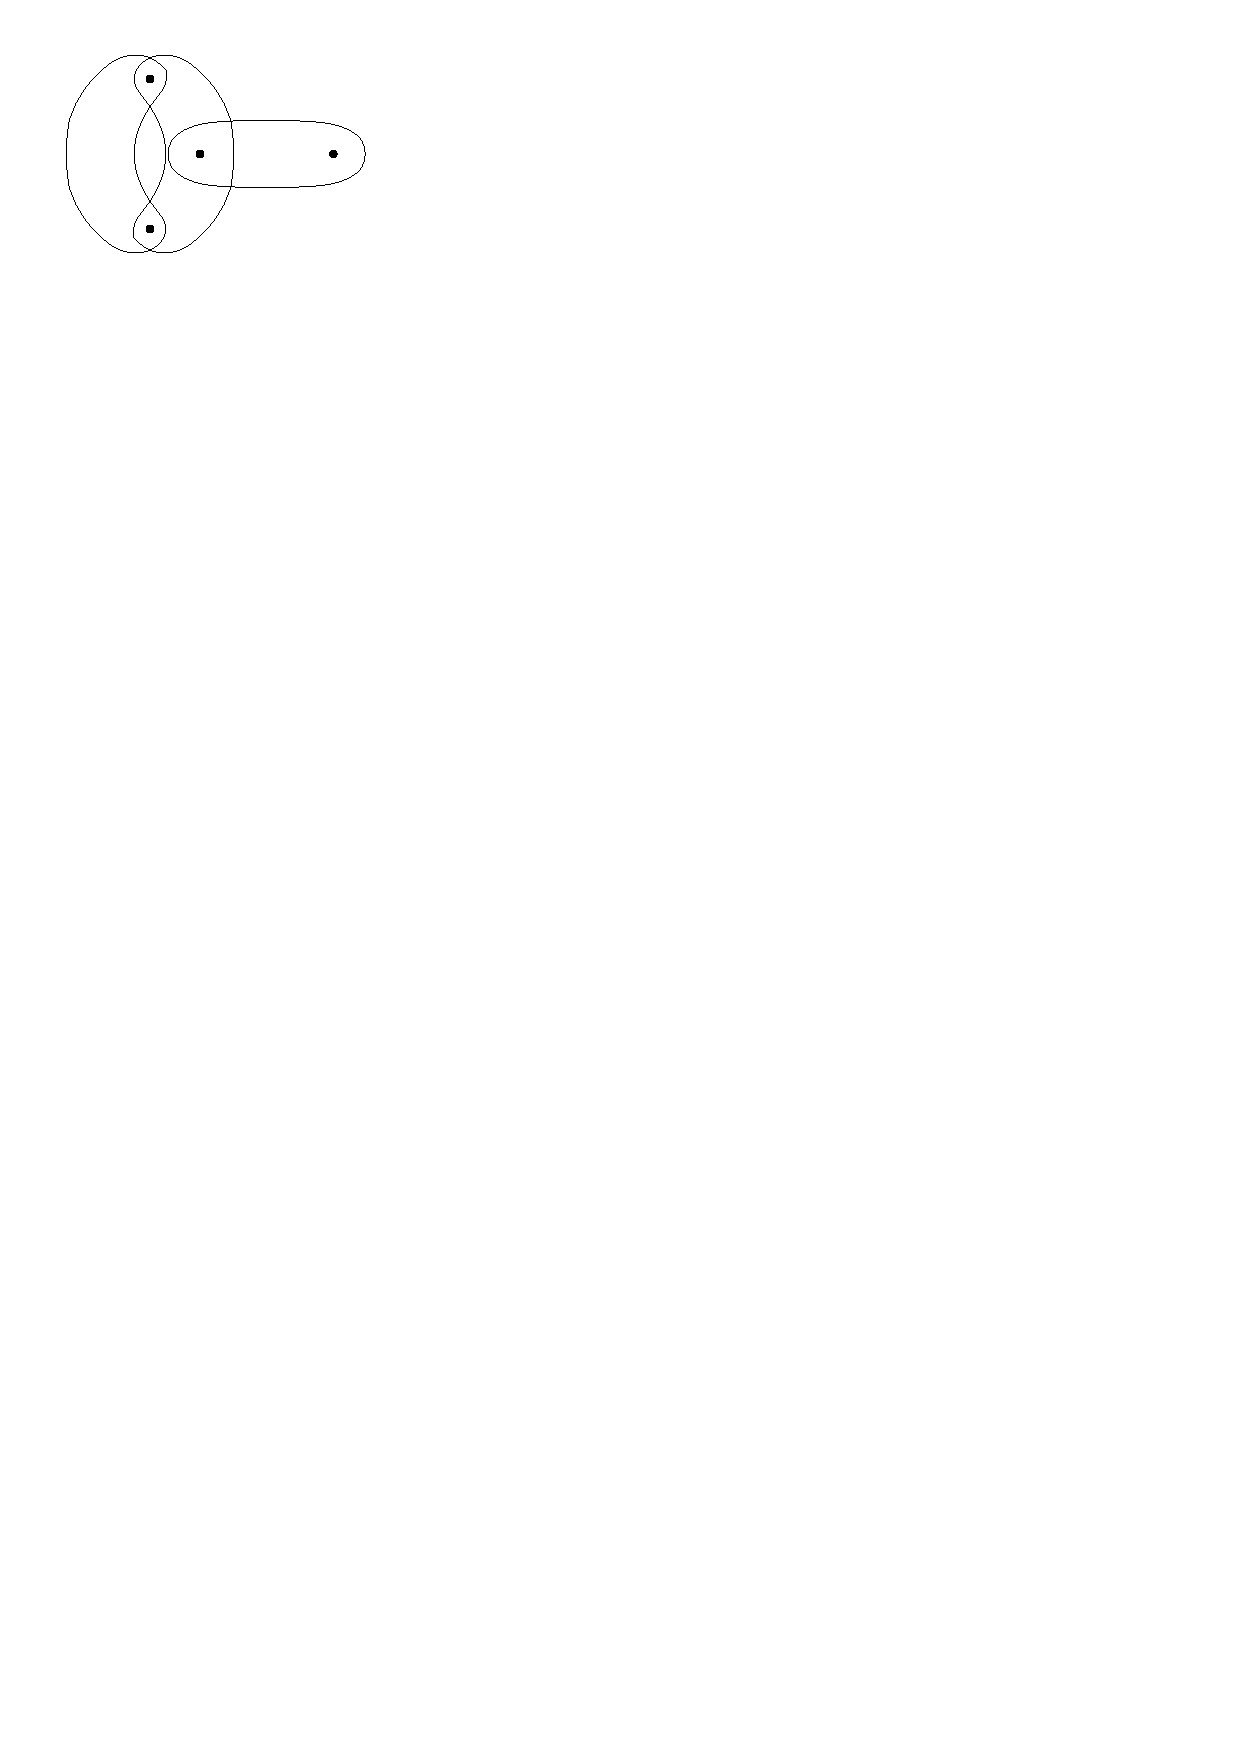
\includegraphics[width=0.7\linewidth]{Graph3edge1.pdf}
		\caption{$\frac{(d-2)!^3}{|Aut(H)|}=\frac{1}{2}
		\left(\frac{d-1}{d-2}\right)$.}
		\end{subfigure}
	\hfill
	\begin{subfigure}{.3\linewidth}
		\centering
		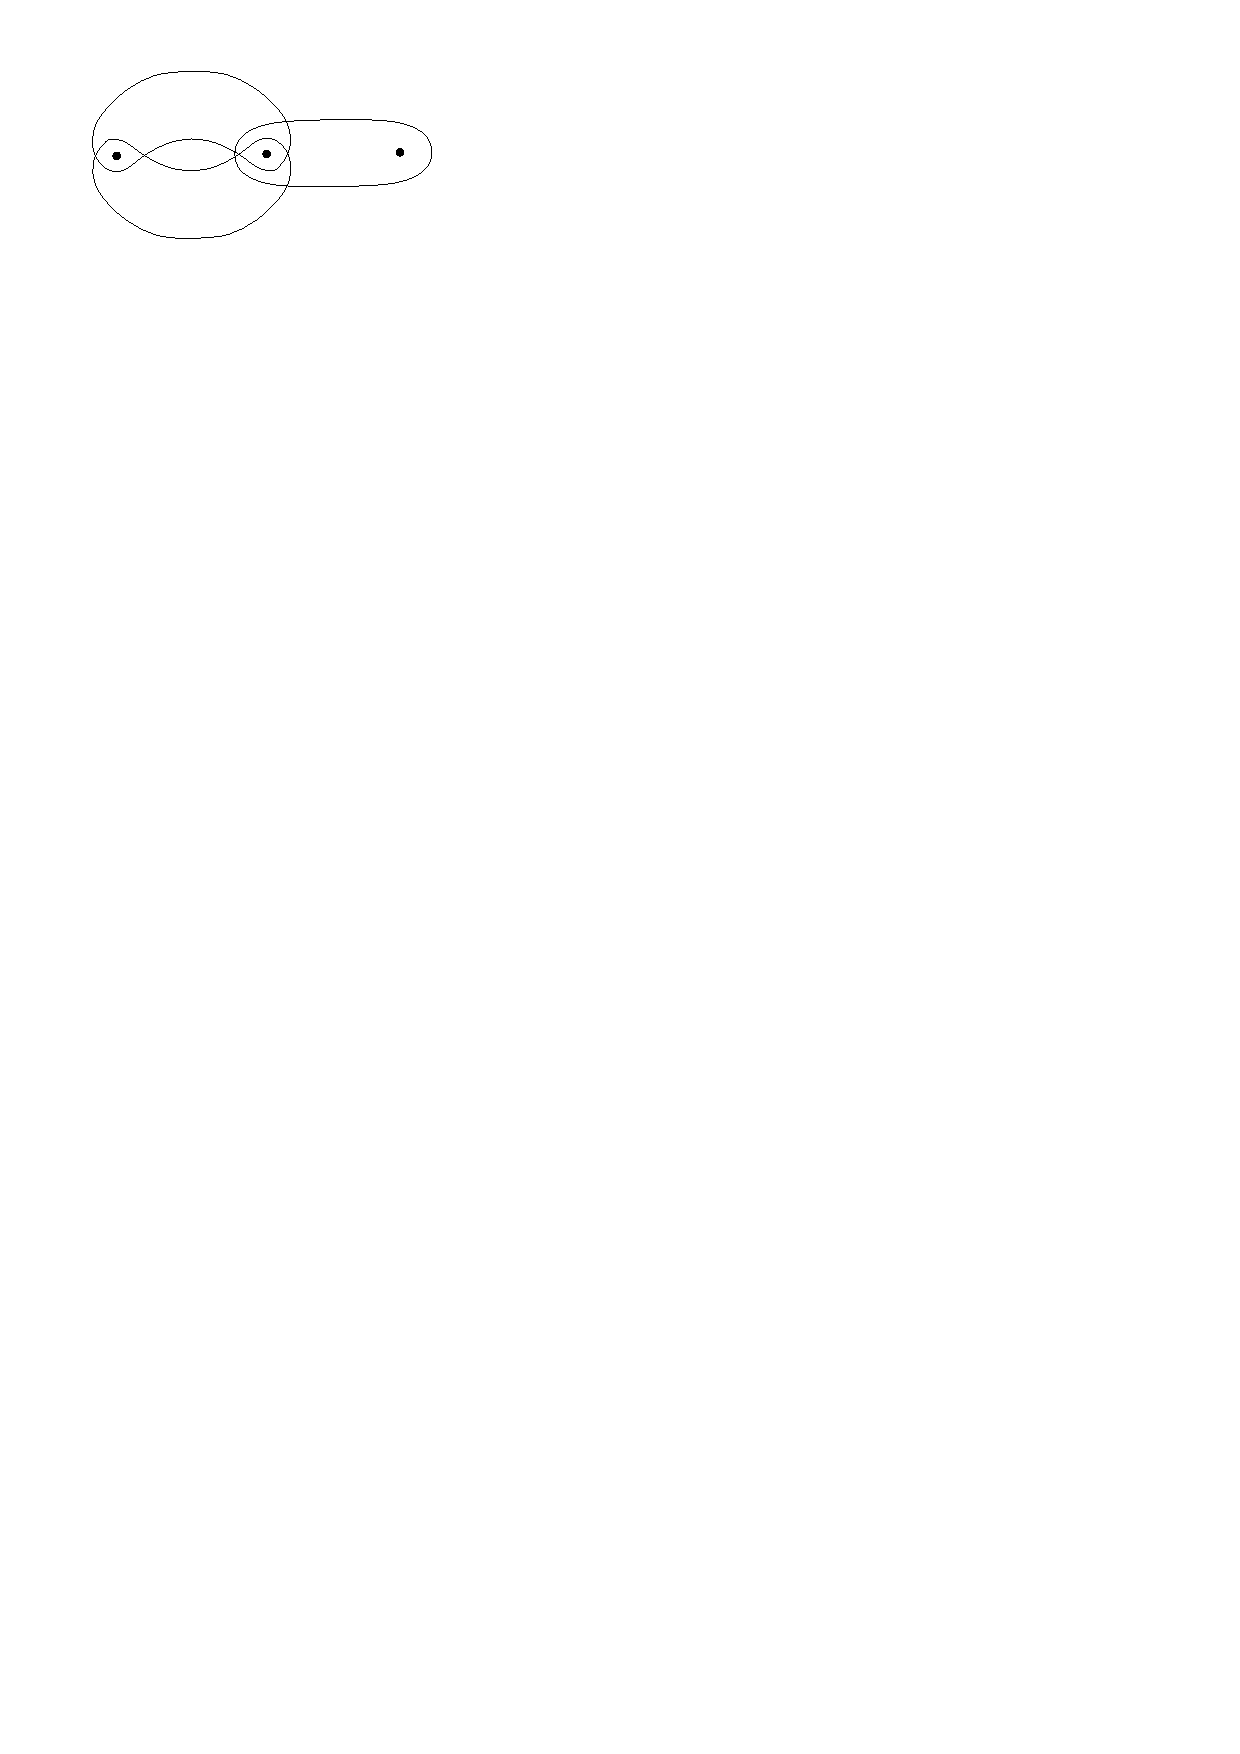
\includegraphics[width=0.8\linewidth]{Graph3edge2.pdf}
		\caption{$\frac{(d-2)!^3}{|Aut(H)|}=\frac{1}{2}
			\left(\frac{1}{d-2}\right)$.}
	\end{subfigure}
	\hfill
	\begin{subfigure}{.3\linewidth}
	\centering
	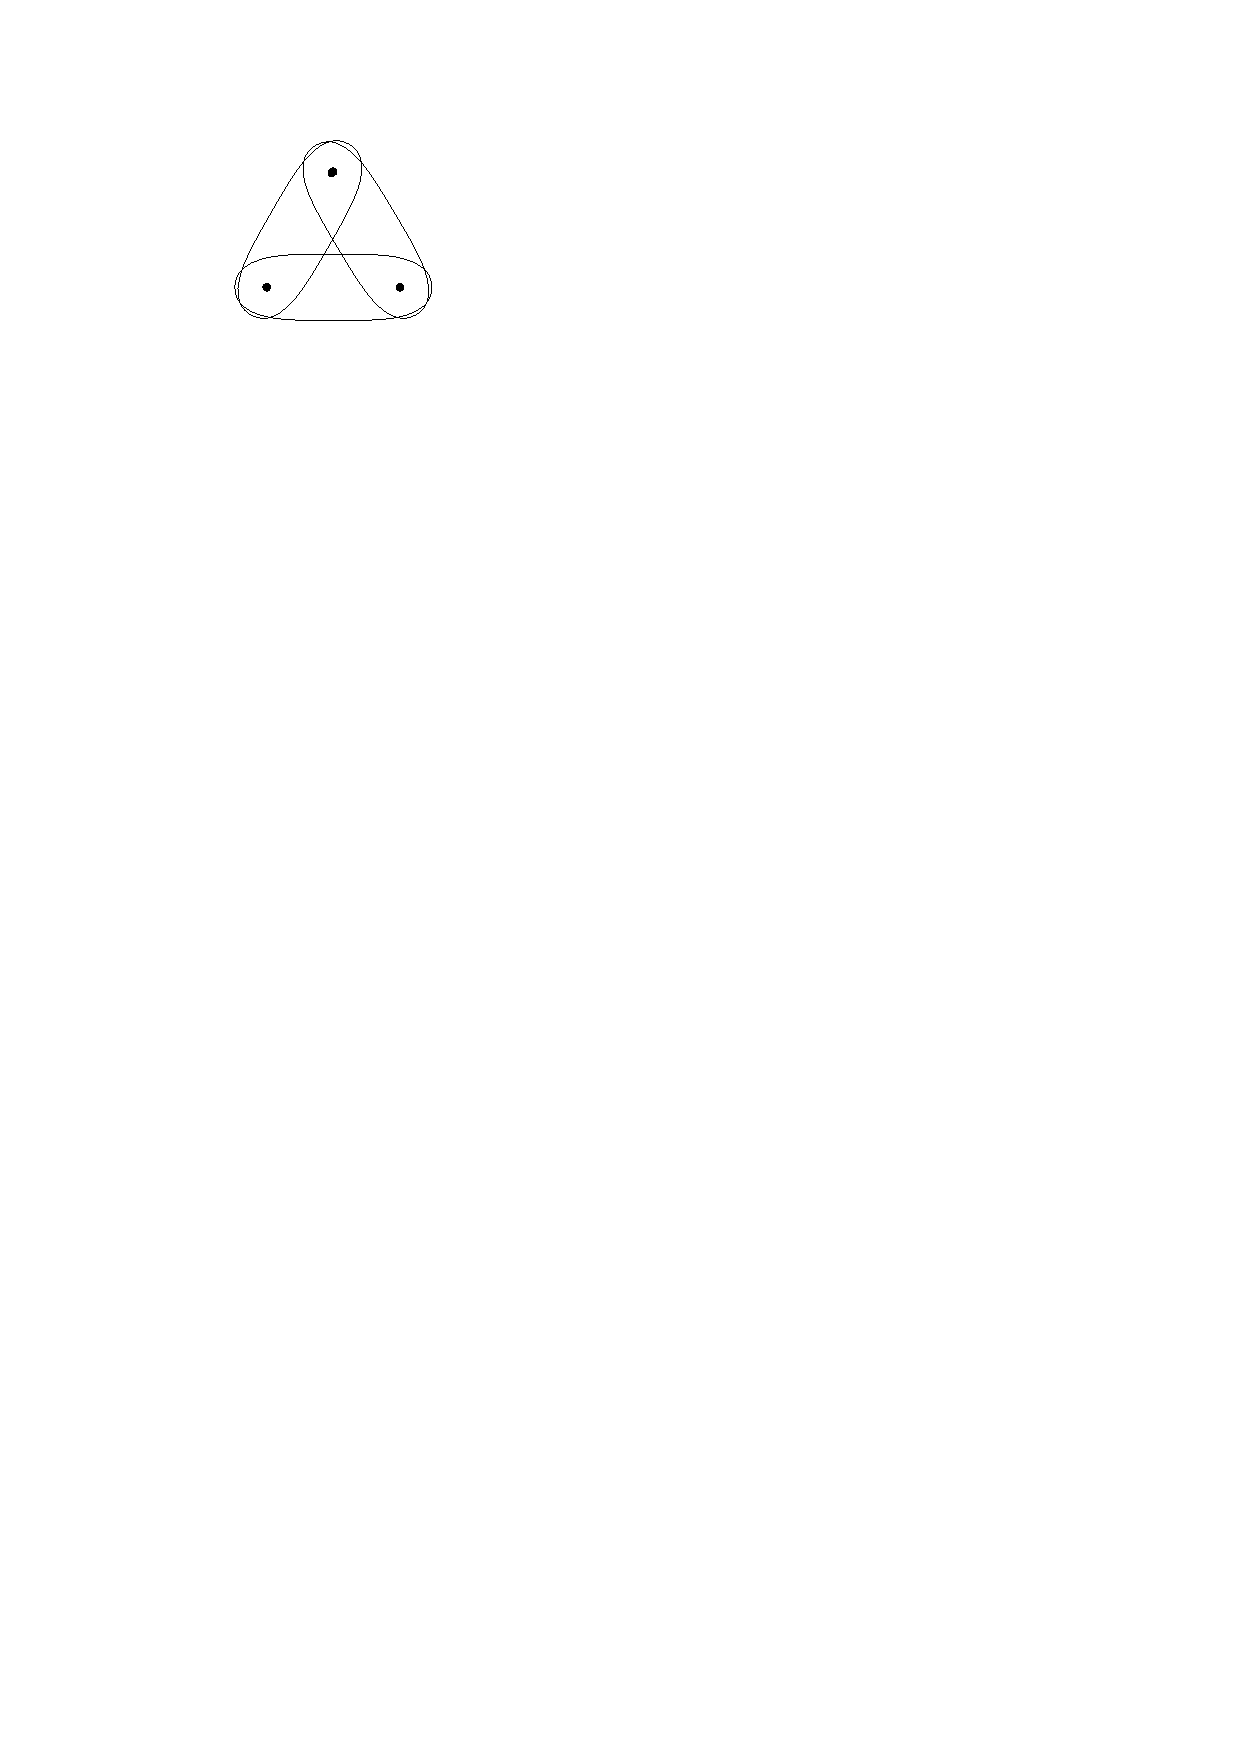
\includegraphics[width=0.6\linewidth]{Graph3edge3.pdf}
	\caption{$\frac{(d-2)!^3}{|Aut(H)|}=\frac{1}{6}
		$.}
	\end{subfigure}
\end{figure}
\par

Using \cref{eqn:cycles} we can bound 
$\sum_{H\in U_l}\frac{(d-2)!^6}{|Aut(H)|}$ by
$\frac{l-2}{2}\left(\frac{d-2}{d-1}\right)$ for $l=4,5$,
and we get
\[
\sum_{j>i}^{q_i}>
s^4\sum_{H\in U_4}\frac{(d-2)!^5}{|Aut(H)|}
+ s^5\sum_{H\in U_5}\frac{(d-2)!^6}{|Aut(H)|}
> \left(\frac{s^42 + s^53}{2}\right) \left( \frac{d-2}{d-1} \right)
> \frac{s^3}{2} \left( \frac{d-2}{d-1} \right)  \geq q_i.
\]
\par
Finally if $H_i$ has only two edges, then $H_i=C_2$,
(here $C_2$ denotes the cycle of length two, as usual) 
and $q_1=s^2\frac{1}{4}$. One can also check, using that
$s\leq 1/e$ and the previous enumeration of unicycles with 
three edges that $q_i=q_1$. 
That is, for any other graph $H\in \mathcal{U}$,
$s^{e(H)}\frac{(d-2)!^{e(H)}}{|Aut(H)|}<\frac{s^2}{4}$.
Let us call $\mathcal{T}$, 
$\mathcal{B}$ and $\mathcal{O}$ to the sets of graphs of the
form $T_{\alpha,\beta}$, $B_{\alpha,\beta}$
and $O_{\alpha,\beta}$ respectively. We have:

\begin{equation} \label{finalbound}
\sum_{j>1} q_j > s^{3}\frac{(d-2)!^{3}}{|Aut(C_3)|}+
\sum_{H\in \mathcal{B}} s^{e(H)}\frac{(d-2)!^{e(H)}}{|Aut(H)|} +
\sum_{H\in \mathcal{O}} s^{e(H)}\frac{(d-2)!^{e(H)}}{|Aut(H)|}.
\end{equation}

We can bound each of the terms in the LHS of last inequality.
Using \cref{eqn:twocycles} we obtain
\[ \sum_{H\in \mathcal{B}} s^{e(H)}\frac{(d-2)!^{e(H)}}{|Aut(H)|}
 =\sum_{k=4}^{\infty} s^k \frac{k-3}{4} \left(\frac{d-2}{d-1}\right)^2.
\]
And using that $s>1/3$, and the fact that for $a,b,c,x\in \R$ and
$|x|<1$ we have
\[
\sum_{n=0}^{\infty}c(a+nb)x^n = 
\frac{ac}{1-x} + \frac{bcx}{(1-x)^2},
\]  
we can get
\begin{equation} \label{finalbound1}
\sum_{H\in \mathcal{B}} s^{e(H)}\frac{(d-2)!^{e(H)}}{|Aut(H)|}=
\sum_{k=5}^{\infty} s^k \frac{k-4}{4} \left(\frac{d-2}{d-1}\right)^2
> s^4 \left(\frac{d-2}{d-1}\right)^2 \frac{9}{16} > s^3 \left(\frac{d-2}{d-1}\right)^2 \frac{3}{16}.
\end{equation}
\par
Analogously as before, using \cref{eqn:cycles} 
and the formula for the arithmetico-geometric series
we get
\begin{equation} \label{finalbound2}
\sum_{H\in \mathcal{O}} s^{e(H)}\frac{(d-2)!^{e(H)}}{|Aut(H)|}
=\sum_{k=3}^{\infty} s^k \frac{k-2}{4} \left(\frac{d-2}{d-1}\right).
> s^3 \left(\frac{d-2}{d-1}\right) \frac{9}{8}
\end{equation}
\par
Now, using  \cref{finalbound1} and \cref{finalbound2} in
\cref{finalbound} an the fact that $\frac{(d-2)!^{3}}{|Aut(C_3)|}
=\frac{1}{6}$ we have
\[
\sum_{j>1} q_j > s^{3}\frac{1}{6} +
s^3 \left(\frac{d-2}{d-1}\right)^2 \frac{3}{16} +
s^3 \left(\frac{d-2}{d-1}\right) \frac{9}{8}.
\]
Finally, substituting 
$\left(\frac{d-2}{d-1}\right)\geq \frac{1}{2}$,
we obtain
\[
\sum_{j>1} q_j > s^{3}\frac{1}{6} +
s^3 \frac{3}{64} +
s^3 \frac{9}{16} = s^3 \frac{32+9+108}{192} > s^3 \frac{3}{4}>
s^2\frac{1}{4}=q_1,
\]
as we wanted. 





 
%We have
%\begin{equation} \label{cyclespaths}
%\sum_{H\in \mathcal{U}_k} \frac{(d-2)!^k}{|Aut(H)|} \geq \
%\sum_{\alpha=2}^{k-1} \frac{(d-2)!^k}{|Aut(O_{\alpha, k-\alpha})|}=
%\begin{cases}
%\frac{(k-3)(d-2)}{d-1} \text{ for } k\geq 4, \\
%\\
%\frac{d-2}{2(d-1)} \text{ for } k=3
%\end{cases} 
%\end{equation}
%\par
%As $1/3 < s < 1/e$, if $k(q_i)\geq 6$ then $k-3\geq 3$ and
%$q_i\leq \sum_{j\geq i} q_j$ because
%\[ \sum_{j\geq i} q_j \geq \sum_{H\in \mathcal{U}_k}
%s^k\frac{(d-2)!^k}{|Aut(H)|} = s^k(k-3) \frac{d-2}{d-1}
%> s^{k-1} \frac{d-2}{d-1} \geq q_i.\]
%\par
%For the case $k(q_i)=5$
%\[ \sum_{j\geq i} q_j \geq \sum_{H\in \mathcal{U}_5}
%s^5\frac{(d-2)!^5}{|Aut(H)|} + \sum_{H\in \mathcal{U}_6}
%s^6\frac{(d-2)!^6}{|Aut(H)|}\geq 
%2 s^5 \frac{d-2}{d-1} + 3 s^6 \frac{d-2}{d-1} >
%3 s^5 \frac{d-2}{d-1} \geq s^4 \frac{d-2}{d-1} \geq q_i.
%\]
%
%For the case $k(q_i)=4$, $e(H_i)\leq 3$, and an enumeration
%of all unicycles with less than $3$ edges gives 
%$q_i\leq \frac{s^3(d-2)}{2(d-1)}$. This way,
%
%\begin{align} \nonumber
%\sum_{j\geq i} q_j \quad & \geq \sum_{k=4}^\infty 
%\sum_{H\in \mathcal{U}_k}
%s^k\frac{(d-2)!^k}{|Aut(H)|}= s^4\frac{d-2}{d-1} 
%\sum_{k=4}^\infty 
%s^{k-4}(k-3) \\
%& \label{arithgeometric}
%>s^4\frac{d-2}{d-1} \sum_{n=0}^\infty 
%3^{-n}(n+1)= s^4\frac{(d-2)}{(d-1)}\frac{9}{4} > 
%\frac{s^3(d-2)}{2(d-1)} \frac{3}{2} > q_i
%\end{align}
%
%Here we have used that the sum of the 
%arithmetic-geometric series
%$\sum_{n=1}^{\infty} bs^{n-1}(a+d(n-1))$ converges to
%$\frac{ab}{1-s} + \frac{dbs}{(1-s)^2}$ when $|s|<1$.
%
%Finally, for $k(i)=3$ the only possible fragment left is
%the cycle of length two. That is, $H_i=C_2$. We have
%$\frac{(d-2)!^2}{|Aut(C_2)|}=\frac{1}{4}$. Consider the sum
%\[  
%\sum_{k=3}^{\infty} \sum_{H\in \mathcal{U}_k} 
%s^k\frac{(d-2)!^k}{|Aut(H)|} =
%\sum_{H\in \mathcal{U}_3} 
%s^3\frac{(d-2)!^3}{|Aut(H)|} +
%\sum_{k=4}^{\infty} \sum_{H\in \mathcal{U}_k}
%s^k\frac{(d-2)!^k}{|Aut(H)|}.
%\]
%We can bound the first term in the following way
%\[
%\sum_{H\in \mathcal{U}_3} 
%s^3\frac{(d-2)!^3}{|Aut(H)|} > s^3\frac{(d-2)!^3}{|Aut(O_{2,1})|} 
%+ s^3\frac{(d-2)!^3}{|Aut(C_3)|}.
%\]
%This is because both $O_{2,1}$ and $C_3$ are non-isomorphic
%members of $\mathcal{U}_3$. The previous $RHS$ equals
%\[s^3\frac{(d-2)}{(d-1)2} 
%+ s^3\frac{1}{6},\]
%and using that $\frac{(d-2)}{(d-1)}\geq \frac{1}{2}$ we get
%that this expression greater or equal than $s^3\frac{5}{12}$.
%We have also the following bound 
%\[\sum_{k=4}^\infty 
%\sum_{H\in \mathcal{U}_k}
%s^k\frac{(d-2)!^k}{|Aut(H)|} > 
%\frac{s^3(d-2)}{(d-1)} \frac{3}{4} \geq s^3 \frac{3}{8}, \]
%where the first inequality had previously been obtained in 
%\cref{arithgeometric} and the second follows again from 
%$\frac{(d-2)}{(d-1)}\geq \frac{1}{2}$. In consequence,
%\begin{align*}  
%\sum_{k=3}^{\infty} \sum_{H\in \mathcal{U}_k} 
%s^k\frac{(d-2)!^k}{|Aut(H)|} &=
%\sum_{H\in \mathcal{U}_3} 
%s^3\frac{(d-2)!^3}{|Aut(H)|} +
%\sum_{k=4}^{\infty} \sum_{H\in \mathcal{U}_k}
%s^k\frac{(d-2)!^k}{|Aut(H)|} \\
%& > s^3 \frac{3}{8} + s^3\frac{5}{12}
%= s^3 \frac{19}{24} > s^2 \frac{19}{72} > s^2\frac{1}{4}=q_i,
%\end{align*}
%as desired.
%	
\end{document}